\documentclass[14pt]{extreport}
\usepackage{gost}
%Тут можно вставить дополнительные пакеты

\begin{document}
\pagestyle{empty} %  выключаем нумерацию
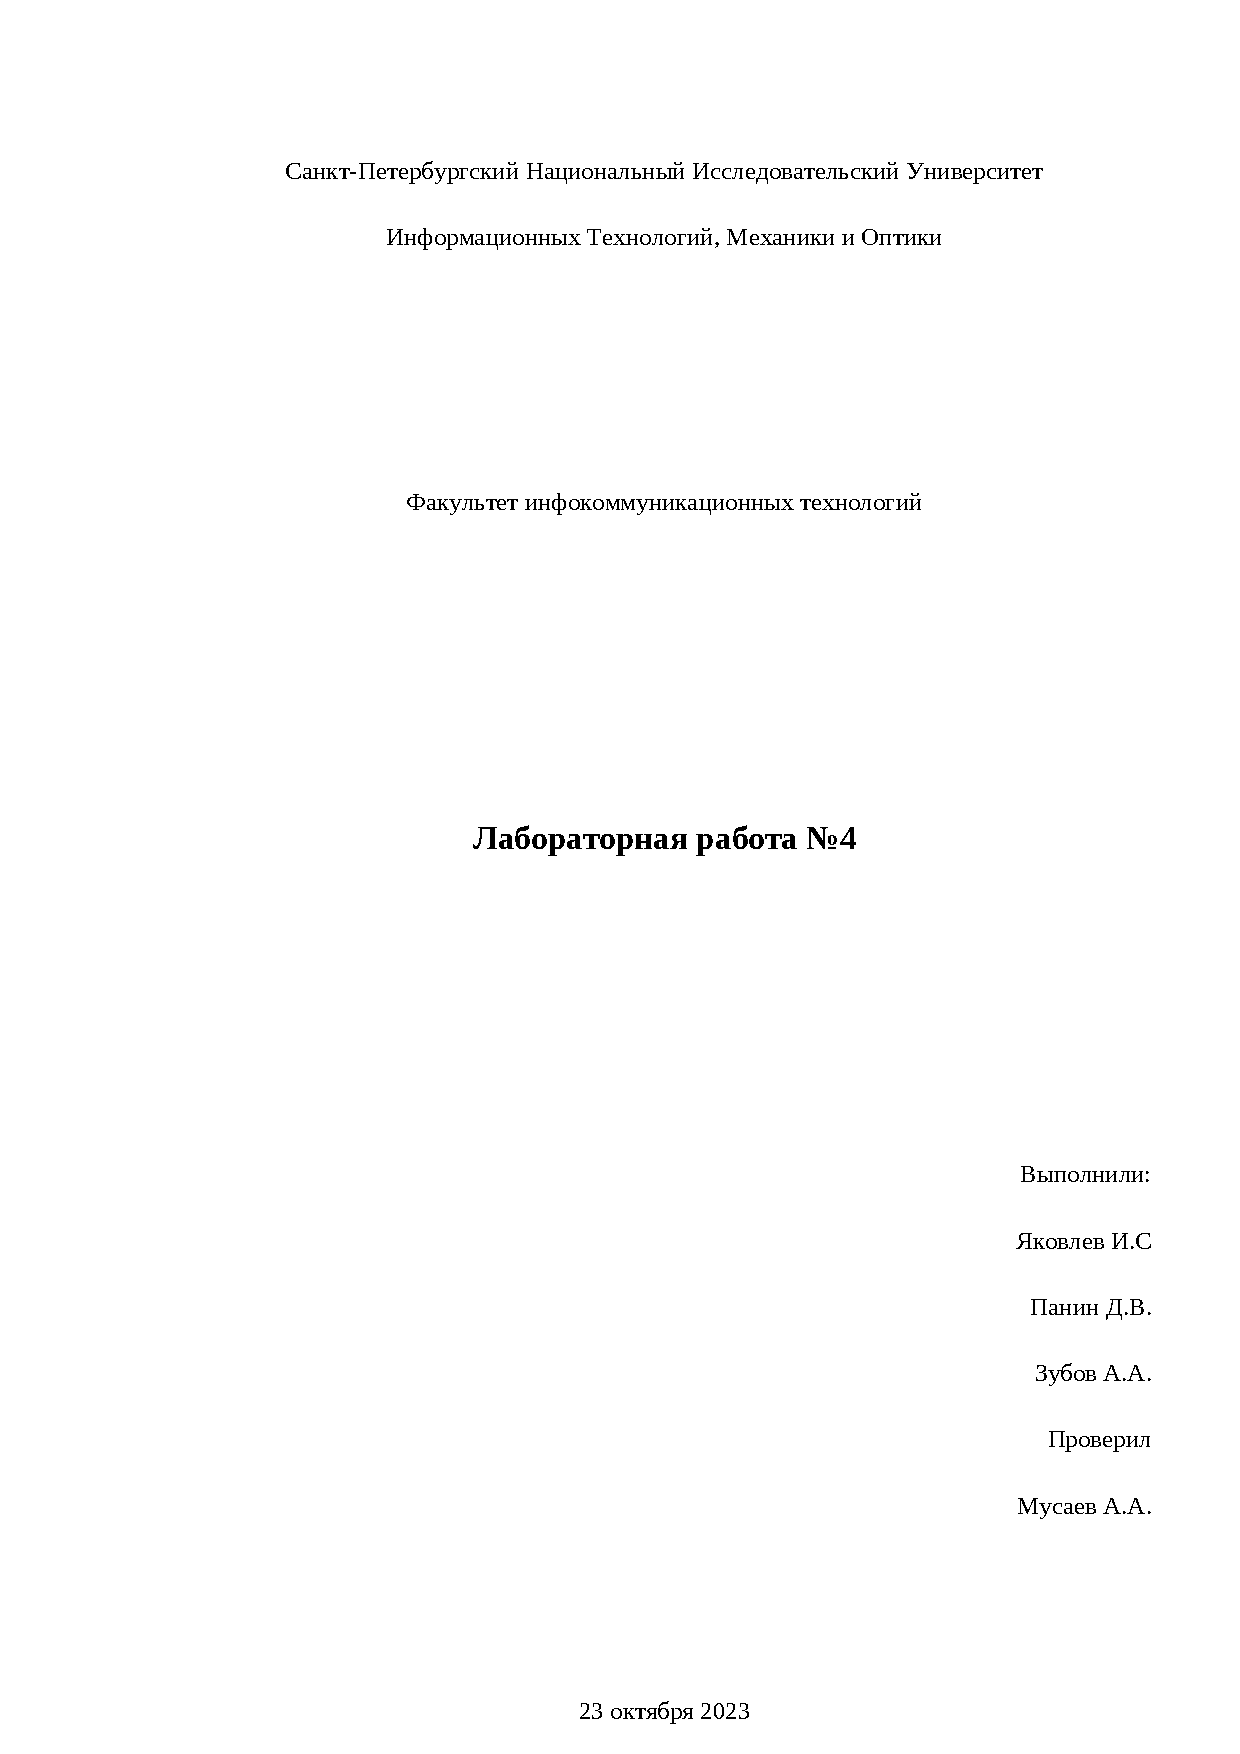
\includepdf[pages=-,pagecommand={}]{Titul.pdf}
\newpage
\phantomsection

\pagestyle{plain} % включаем нумерацию  

\tableofcontents
\newpage
\phantomsection

\intro

Это отчет о выполнении лабораторной работы №4. В первой главе представлен решение первой задачи - реализация алгоритма проверки скобочной последовательности на правильность. Во второй главе представлено решение второй задачи - составлен граф петербургского метро и реализован алгоритм поиска кротчайшего пути от одной станции к другой. В третьей главе представлено решение третьей задачи - реализация алгоритма поиска выхода из лабиринта.


\chapter{Задание --- Реализация проверки скобочной последовательности}


\begin{figure}[H]
\center{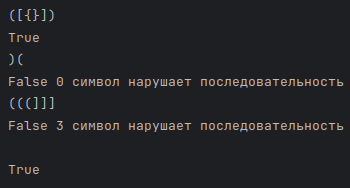
\includegraphics[width=0.9\linewidth]{1_task.png}}
\caption{1 task output}
\label{grf1}
\end{figure}

Был написан алгоритм проверяющий скобочную последовательность, содержащую три вида скобок. Алгоритм работает верно, выводит номер первой неправильной скобки (нумерация скобок с 0).


\newpage

\chapter{Задание --- Кратчайший путь метро СПБ}

\begin{figure}[H]
\center{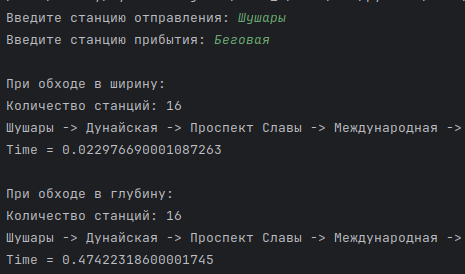
\includegraphics[width=0.9\linewidth]{2_task.png}}
\caption{2 task output}
\label{grf2}
\end{figure}

Была перенесена карта станций метро СПБ в граф (список смежности). Написан алгоритм поиска минимального пути между станциями с помощью поиска в ширину и поиска в глубину. Также проанализирована скорость работы каждого с помощью модуля timeit. Как мы можем видеть алгоритм поиска в ширину работает сильно быстрее при решении этой задачи. 

Вывод о выборе нужного алгоритма:

Если мы решаем задачу поиска кратчайшего пути в невзвешенном графе, то эффективней будет использовать поиск в ширину, однако алгоритм поиска в глубину будет эффективней в задачах на поиск всех путей до точки, генерацию всех подмножеств, использование топологической сортировки и поиск в глубину в графах с циклами.


\chapter{Задание --- Реализация алгоритма поиска выхода из лабиринта}


\begin{figure}[H]
\center{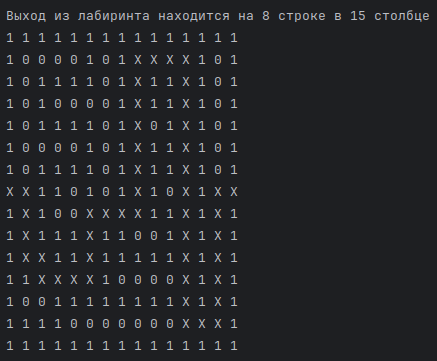
\includegraphics[width=0.9\linewidth]{3_task.png}}
\caption{3 task output}
\label{grf2}
\end{figure}

 Алгоритм пройденный путь помечает крестиками, как мы видим путь найден верно, и выведены координаты выхода. Если бы выхода не было, то алгоритм бы вывел, что выхода нет.

\newpage

\begin{figure}[H]
\center{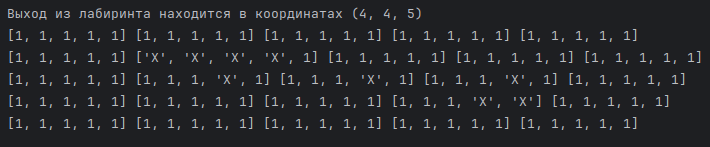
\includegraphics[width=0.9\linewidth]{3_task_xyz.png}}
\caption{3 task output xyz}
\label{grf2}
\end{figure}

Также реализован алгоритм для трёхмерно пространства, ссылка на страничку с кодом в заключении.

Пример был взят для лабиринта размерности 5, так как писать пример для трёхмерного пространства 15x15x15 довольно долго.

\newpage
\phantomsection
\conclusions

В ходе решения этой лабораторной работы было:
\begin{itemize}
    \item Написан алгоритм проверки скобочной последовательности на правильность;
    \item Перенесена карта метро СПБ и реализован алгоритм поиска кратчайшего пути между станциями;
    \item Оценена скорость алгоритмов поиска в ширину и поиска в глубину, на данной задаче;
    \item Реализован алгоритм поиска пути в лабиринте.
\end{itemize}

Github с кодами программ --- \url{https://github.com/alekos-bigo/aisd-labs/tree/main/lab-4}

\newpage
\begin{thebibliography}{99}

\bibitem{bib1} Alfred V. AHO, Jhon E. Hopkroft, Jeffrey D. Ullman Структуры данных и алгоритмы. --- Alfred V. AHO, Jhon E. Hopkroft, Jeffrey D. Ullman. Москва, Санкт-Петербург, Киев: Издательский дом "Вильямс". 2003.

\end{thebibliography}

\end{document}

